\documentclass[a4paper,14pt]{article}

\usepackage{comment} % Para comentar várias linhas ao mesmo tempo

%matemática
\usepackage{amsmath}
\usepackage{amssymb}

%diagramação
\usepackage{extsizes}
\everymath{\displaystyle}
\usepackage{geometry}
\usepackage{fancyhdr}
\usepackage{multicol}
\usepackage{graphicx}
\usepackage[brazil]{babel}
\usepackage[shortlabels]{enumitem}
\usepackage{cancel}
\usepackage{textcomp}
\usepackage{tcolorbox}

%tabelas
\usepackage{array} % Para melhor formatação de tabelas
\usepackage{longtable}
\usepackage{booktabs}  % Para linhas horizontais mais bonitas
\usepackage{float}   % Para usar o modificador [H]
\usepackage{caption} % Para usar legendas em tabelas
\usepackage{wrapfig} % Para usar tabelas e figuras flutuantes


%tikzpicture
\usepackage{tikz}
\usepackage{scalerel}
\usepackage{pict2e}
\usepackage{tkz-euclide}
\usetikzlibrary{calc}
\usetikzlibrary{patterns,arrows.meta}
\usetikzlibrary{shadows}
\usetikzlibrary{external}

%pgfplots
\usepackage{pgfplots}
\pgfplotsset{compat=newest}
\usepgfplotslibrary{statistics}
\usepgfplotslibrary{fillbetween}

%colours
\usepackage{xcolor}



\columnsep=2cm
\hoffset=0cm
\textwidth=8cm
\setlength{\columnseprule}{.1pt}
\setlength{\columnsep}{2cm}
\renewcommand{\headrulewidth}{0pt}
\geometry{top=1in, bottom=1in, left=0.7in, right=0.5in}

\pagestyle{fancy}
\fancyhf{}
\fancyfoot[C]{\thepage}

\begin{document}
	
	\noindent\textbf{6FMA80 - Matemática} 
	
	\begin{center}Multiplicação de inteiros (Versão estudante)
	\end{center}
	
	\noindent\textbf{Nome:} \underline{\hspace{10cm}}
	\noindent\textbf{Data:} \underline{\hspace{4cm}}
	
	%\section*{Questões de Matemática}
	
	\begin{multicols}{2}
		\noindent A multiplicação de qualquer número inteiro $x$ por 0 é sempre igual a 0, isto é, se $x \in \mathbb{Z}$, $0 \cdot x = x \cdot 0 = 0$ \\
		Multiplicar um número inteiro $x$ por -1 é o mesmo que tomar o oposto de $x$, ou seja, $(-1) \cdot x = -x$. \\
		As seguintes regras são sempre válidas: 
		\begin{itemize}
			\item Positivo vezes positivo é positivo.
			\item Positivo vezes negativo é negativo.
			\item Negativo vezes positivo é negativo.
			\item Negativo vezes negativo é positivo.
		\end{itemize}
		\noindent\textsubscript{-----------------------------------------------------------------------}
		\begin{enumerate}
			\item Efetue.
			\begin{enumerate}[a)]
				\item $6 \cdot (-4)$ \\\\\\\\
				\item $8 \cdot (-9)$ \\\\\\\\
				\item $0 \cdot 40$ \\\\\\\\
				\item $10 \cdot (-3)$ \\\\\\\\
				\item $5 \cdot (-1)$ \\\\\\\\
				\item $1 \cdot (-7)$ \\\\\\\\
				\item $(-4) \cdot 0$ \\\\\\\\
				\item $0 \cdot 0$ \\\\\\\\
				\item $7 \cdot 7$ \\\\\\\\
			\end{enumerate}
			\item Dado $x$, desenhe na reta:
			\begin{enumerate}[a)]
				\item $(-6)x$ \\\\
				\begin{tikzpicture}
					% Desenha a reta
					\draw[thick] (0,0) -- (6.5,0); % Reta horizontal de (0,0) a (6.5,0) com 9 pontos
					% Desenha os círculos nos pontos da reta
					\foreach \x in {5.28, 5.94} { % Para cada ponto em {8, 9}
						\fill (\x, 0) circle (3pt); % Desenha um círculo de raio 3pt em (x, 0)
						% Adiciona legendas nos pontos específicos
						\node at (5.28, -0.4) {0};   % Legenda "0" no oitavo ponto
						\node at (5.94, -0.4) {x};    % Legenda "x" no nono ponto
					}
				\end{tikzpicture} 
				\item $4x$ \\\\
				\begin{tikzpicture}
					% Desenha a reta
					\draw[thick] (0,0) -- (6.5,0); % Reta horizontal de (0,0) a (6.5,0) com 9 pontos
					% Desenha os círculos nos pontos da reta
					\foreach \x in {4.62, 5.94} { % Para cada ponto em {7, 9}
						\fill (\x, 0) circle (3pt); % Desenha um círculo de raio 3pt em (x, 0)
						% Adiciona legendas nos pontos específicos
						\node at (4.62, -0.4) {x};   % Legenda "x" no sétimo ponto
						\node at (5.94, -0.4) {0};    % Legenda "0" no nono ponto
					}
				\end{tikzpicture} 
			\end{enumerate}
			\item Observemos que, se $x$ é inteiro, então, por exemplo, $3x$ é igual a $x + x + x$. Escreva como soma os produtos abaixo, em que as letras representam números inteiros.
			\begin{enumerate}[a)]
				\item $2a$ \\\\\\\\
				\item $6k$ \\\\\\\\
				\item $9y$ \\\\\\\\	
			\end{enumerate}
			\item Efetue.
			\begin{enumerate}[a)]
				\item $28 \cdot 63$ \\\\\\\\
				\item $(-67) \cdot 92$ \\\\\\\\
				\item $54 \cdot (-66)$ \\\\\\\\
				\item $(-39) \cdot (-81)$ \\\\\\\\
				\item $(-8) \cdot 5$ \\\\\\\\
				\item $(-31) \cdot (-41)$ \\\\\\\\
			\end{enumerate}
			%23 a 25
			\item Na reta abaixo, estão representados $x$ e $y \cdot x$. \\
			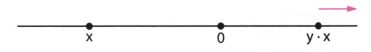
\includegraphics[width=1\linewidth]{6FMA80_imagens/imagem1}
			
			Diga se são positivos, negativos ou nulos cada um dos números abaixo. Justifique sua resposta.
			\begin{enumerate}[a)]
				\item $x$
				\item $y \cdot x$
				\item $y$
				\item $y^2 \cdot x$
				\item $2y \cdot x$
				\item $0 \cdot x$
				\item $y \cdot x \cdot 0$
			\end{enumerate}
			\item Efetue:
			\begin{enumerate}[a)]
				\item $(-2) \cdot 7$ \\\\\\\\
				\item $3 \cdot (-6)$ \\\\\\\\
				\item $51 \cdot 0$ \\\\\\\\
				\item $12 \cdot (-3)$ \\\\\\\\
				\item $(-1) \cdot (-9) \cdot 1$ \\\\\\\\
				\item $(-9) \cdot 1$ \\\\\\\\
				\item $(-7) \cdot 0$ \\\\\\\\
				\item $9 \cdot (-4)$ \\\\\\\\
				\item $7 \cdot 6$ \\\\\\\\
				\item $(-7) \cdot 4$ \\\\\\\\
				\item $(-15) \cdot (-53)$ \\\\\\\\
				\item $(-16) \cdot 6$ \\\\\\\\
				\item $(-19)(-21)$ \\\\\\\\
				\item 
			\end{enumerate}
		\end{enumerate}
		$~$ \\ $~$ \\
	\end{multicols}
\end{document}